\documentclass[SDSUThesis.tex]{subfiles} 
\begin{document}

% All about the SDLC Analytic Engine
\section{SDLC ANALYTIC ENGINE}

In order for an SDO to properly track the elements of MPI, a data storage system should be available to store the appropriate data.   This storage system will be named the SDLC Analytic Engine (SDLC-AE). Figure \ref{fig:sdlc-ae} provides an overview of the data that could potentially be stored in the SDLC-AE.

The SDLC-AE would make gamification of the SDLC attainable.  Prior attempts
at gamification of the SDLC focus only on the development phase \cite{Dubois2013} \cite{Snipes2013}.

\begin{figure}[ht]
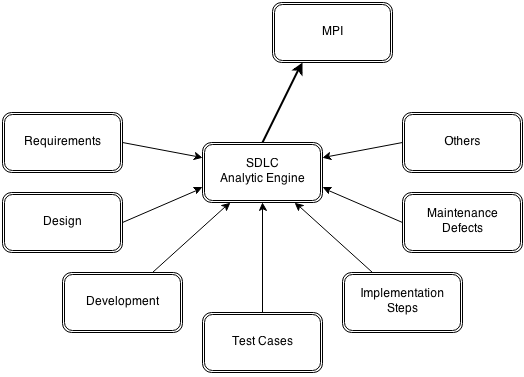
\includegraphics[scale=.7]{images/sdlc-ae.png}
\caption{SDLC Analytic Engine}
\label{fig:sdlc-ae}
\end{figure}

\subsection{DATABASE STRUCTURE}
   All the data necessary to compute MPI needs to be stored in a database.  This section will 
   layout the structure of tables and relationships necessary to the store all the data
   within a relational database such as MySQL or PostgreSQL.  Eventually,
   database diagrams and SQL scripts will be provided in the section.

\subsection{QUERIES}
    The section will provide the necessary SQL queries to obtain the correct data
    needed to compute the individual elements of MPI.
    
\subsection{COMPUTATIONS}
    This section will provide R scripts to calculate each individual score and the overall 
    MPI score. The scripts will need to be run every time the data is updated and the MPI
    score needs to be recalculated.


    \subsection{ESTIMATION}
    
    \begin{itemize}
    \item Change to Database Structure  
    \item Modify Database Data    
    \item Create a New Database, number of new databases  
    \item Server Configuration Changes Required   
    \item New Servers Required   
    \item Number of Team Members Involved  
    \item Number of (sub)Systems Involved  
    \item Estimation Date
    \item Number of Days Allowed
    \item List of Other Attributes
    \item Number of Screens Involved 
    \item Actual Value (hours, days, dollars) 
    \end{itemize}
    
    
    Estimated Dev Hours - The number of development hours estimated for a project, this is just developer hours
    Estimated Doc Hours - The number of documentation hours estimated for a project
    Estimated Test Hours - The number of testing hours estimated for a project
    Estimated Deployment Hours - The number of estimated hours required to deploy the project
    
    \subsection{REQUIREMENTS}
    List of: 
    \begin{description}
      \item[Title] 
      \item[Descrition]
      \item[author]
      \item[projectID]
      \item[date]
      \item[Comments] list of \\
      \begin{description}
        \item[date]
        \item[comment Text]
        \item[author]
      \end{description}
    \end{description}
    
    \subsection{MAINTENANCE (DEFECTS)}
    List of:
    \begin{description}
      \item[Project] 
      \item[Release]
      \item[description]
      \item[date Entered]
      \item[Date fixed]
      \item[Comments] list of \\
      \begin{description}
        \item[date]
        \item[comment Text]
        \item[author]
      \end{description}
    \end{description}
    
    
    
    \subsection{TESTING}
    
    List of:
    \begin{description}
      \item[Project] 
      \item[Release]
      \item[title]
      \item[description]
      \item[author]
      \item[Date Started]
      \item[Date Executed]
      \item[Status (Pending, pass, fail)]
      \item[Comments] list of \\
      \begin{description}
        \item[date]
        \item[comment Text]
        \item[author]
      \end{description}
    \end{description}
    
    \subsection{DEVELOPMENT}
    
    List of Coding Tasks:
    \begin{description}
      \item[Project] 
      \item[Release]
      \item[List of Files]
      \item[author]
      \item[Date Started]
      \item[Completion Date]
      \item[Number of Unit Tests]
      \item[Lines of Code]
      \item[Others] See \cite{Jones2009, Jones2012, Rubin2007, Snipes2013}
    \end{description}
    
    \subsection{IMPLEMENTATION}
    
    List of:
    \begin{description}
      \item[Project] 
      \item[Release]
      \item[date Entered]
      \item[Date Scheduled]
      \item[Date Executed]
      \item[Ordering/Prerequisites]
      \item[Comments] list of \\
      \begin{description}
        \item[date]
        \item[comment Text]
        \item[author]
      \end{description}
    \end{description}


\end{document}







